\documentclass[a4paper,numbers=noenddot,DIV=calc]{scrbook} %appendixprefix=true,chapterprefix=true
%\usepackage{scrpage2} % para cabeçalhos, automático em livros
\usepackage{fontspec}
\defaultfontfeatures{Ligatures={TeX}}
\setmainfont{Minion Pro}
\setsansfont{Myriad Pro}
\setmonofont[Scale=.9]{Consolas}
\usepackage{polyglossia}
\setmainlanguage{brazil}
\setotherlanguages{french,english,german,russian,greek,spanish,italian,norsk}
\usepackage[tocgraduated]{tocstyle}
\usetocstyle{nopagecolumn}
\usepackage{graphicx}
\usepackage[marginal]{footmisc}
\usepackage{enumerate}
\usepackage[bookmarks]{hyperref}
\usepackage[dvipsnames]{xcolor}
\usepackage[xcolor]{mdframed}
\usepackage{lipsum}

\title{Título}
\subtitle{Um exemplo de livro} %subtítulo
\author{Autor}
\date{Data}
\publishers{Editora Virtual Imhotep, Ltda.} %editora



%\pagestyle{plain} %retire o % se quiser só números de página, sem cabeçalhos.

\begin{document}

\frenchspacing

\maketitle

\frontmatter

\tableofcontents % comente ( % na frente) se não quiser sumário
\listoffigures % comente ( % na frente) se não houver figuras
%\listoftables % descomente (retire o %)se quiser lista de tabelas

%Use \% para porcento; \& para &. Dê espaço de uma linha entre dois parágrafos.
%Use \emph{texto} para itálico.
%Seja feliz.

\mainmatter

\addchap{Introdução}

\chapter{Capítulo}


\section{Coloque o título da seção}
\lipsum[1-5]


\begin{figure}
\centering
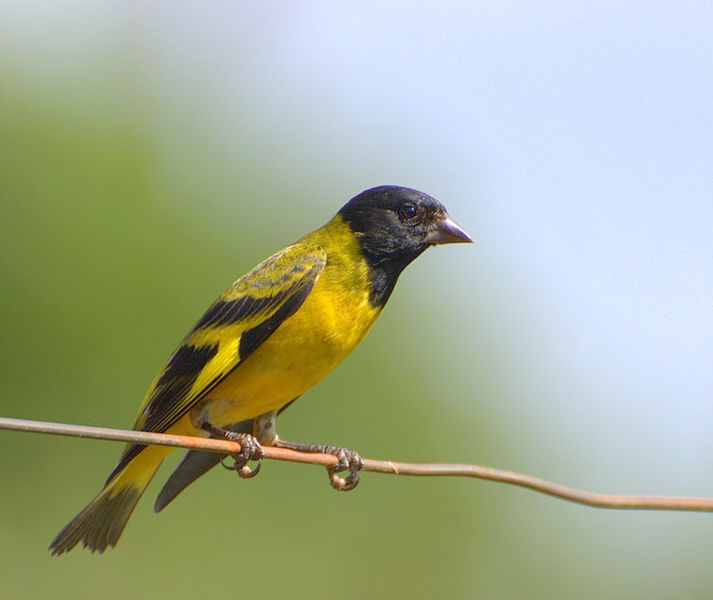
\includegraphics[width=0.5\linewidth]{pintassilgo}
\caption{Pintassilgo-de-cabeça-preta. \textit{Carduelis magellanica}.}
\label{pintassilgo}
\end{figure}


\chapter{Capítulo}

\section{Coloque o título da seção}
\lipsum[1]

\subsection{Subseção}

\lipsum[1-5] %só para preencher com texto sem sentido.


\chapter{Capítulo}
\section{Coloque o título da seção}
\lipsum[1-5]

\addchap{Bibliografia}

\setlength{\parindent}{0pt}

Schimmel, Annemarie, and Stuart Cary Welch. \textit{Anvari's Divan: A Pocket Book for Akbar}.  New York: The Metropolitan Museum of Art, 1983.

\setlength{\parskip}{10pt} %acrescente depois da primeira entrada bibliográfica

Mearsheimer, John. \textit{The Tragedy of Great Power Politics.} New York and London: W.W. Norton \& Company, 2001.




\end{document}
